\documentclass[UTF8]{ctexart}
\usepackage{graphicx}
\usepackage{amsmath}
\usepackage{amssymb}
\usepackage{hyperref}
\date{}
\title{Kalman Filter 基础知识}
\begin{document}

\maketitle

\section{卡尔曼滤波简介}
本小节\footnote{为了与常规用法一致,本节使用 $x$ 代表状态。}先简要介绍卡尔曼滤波(Kalman Filtering,简称:KF),下一小节将介绍 EKF 并将其用于参数的学习。
关于 KF 和 EKF 的详细描述可参阅文献:
[1]SIMON D. Optimal state estimation: Kalman, H [infinity] and nonlinear approaches[M]. Hoboken, N.J: Wiley-Interscience, 2006.


KF 可以由递归最小二乘(RLS)简单扩展得到。
在 LS 中,测量的增多会导致极大的计算量,而 RLS 则可以递归地对状态进行估计。即,对于一个状态恒为 $x$ 的系统,其测量方程为:
\begin{equation}
  \label{eq:rls_observe}
  y_k =H_kx + v_k
\end{equation}
式中,$y_k$ 为 $k$ 时刻的测量值,$H_k$ 为 $k$ 时刻的测量矩阵,$v_k$ 为测量误差,其协方差矩阵记为 $R_k$。
RLS 的目标是寻找 $k$ 时刻的增益矩阵 $K_k$,使得 $k$ 时刻的状态估计 $\hat{x}_k$ 与 $k-1$ 时刻的状态估计 $\hat{x}_{k-1}$ 满足:
\begin{equation}
  \label{eq:12}
  \hat{x}_k =\hat{x}_{k-1}+K_k(y_k-H_k\hat{x}_{k-1})
\end{equation}
若以 $\epsilon_{x,k}=x-\hat{x}_k$ 代表 $k$ 时刻的估计误差,$P_k=E(\epsilon_{x,k}\epsilon_{x,k}^T)$ 代表此刻的估计误差协方差矩阵,则最小化目标函数 $Tr(P_k)$\footnote{$E[(x_1-\hat{x}_1)^2+\ldots+(x_n-\hat{x}_n)^2]=E[\epsilon_{x_1,k}^2+\ldots+\epsilon_{x_n,k}^2]=E[\epsilon_{x,k}^T\epsilon_{x,k}]=E[Tr(\epsilon_{x,k}\epsilon_{x,k}^T)]=Tr(P_k).$}可得\footnote{此处亦可理解为 RLS 的测量更新方程。}:
\begin{align}
K_k&=P_{k-1}H^T_k(H_kP_{k-1}H^T+R_k)^{-1} \\
P_k&=(I-K_kH_k)P_{k-1}(I-K_kH_k)^T+K_kR_kK_k^T
\end{align}

若放松 RLS 中状态 $x$ 恒定的假设,令:
\begin{equation}
x_k=F_{k-1}x_{k-1}+G_{k-1}u_{k-1}+\omega_{k-1}
\end{equation}
式中,$u_k$ 为已知输入,$\omega_k$ 为协方差为 $Q_k$ 的零均值高斯白噪声。
此时,\eqref{eq:rls_observe} 亦变为:
\begin{equation}
  y_k =H_kx_k + v_k
\end{equation}
那么,状态 $x_k$ 的均值的更新方程及其协方差的时间更新方程为:
\begin{align}
  \label{eq:rls_relaxed_x}
  \bar{x}_k &=F_{k-1}\bar{x}_{k-1}+G_{k-1}u_{k-1}\\
  \label{eq:rls_relaxed_p}   
  P_{k}&=F_{k-1}P_{k-1}F_{k-1}^T+Q_{k-1}        
\end{align}

在卡尔曼滤波(KF)的推导中,为了突出时间更新和测量更新,对测量前后状态相关的值加以区分:$\hat{x}_k^-$ 表示 $k$ 时刻的测量值到来之前对状态 $x_k$ 的估计值,$\hat{x}_k^+$ 表示考虑 $k$ 时刻的测量值 $y_k$ 后对状态 $x_k$ 的重新估计值。
相应地,$P_k^-$ 表示 $\hat{x}_k^-$ 的估计误差的协方差,$P_k^+$  表示 $\hat{x}_k^+$ 表示 $\hat{x}_k^+$ 的估计误差的协方差,即:
\begin{align}
  P_k^-&=E[(x_k-\hat{x}_k^-)(x_k-\hat{x}_k^-)^T]\\ 
  P_k^+&=E[(x_k-\hat{x}_k^+)(x_k-\hat{x}_k^+)^T] 
\end{align}
而 KF 的递推公式只需要在 RLS 的基础上稍加更改并结合 \eqref{eq:rls_relaxed_x} 和 \eqref{eq:rls_relaxed_p} 得到。
KF 的\emph{时间更新方程}为:
\begin{align}
  \hat{x}_k^- &=F_{k-1}\hat{x}_{k-1}^++G_{k-1}u_{k-1}\\
  P_{k}^- &=F_{k-1}P_{k-1}^+F_{k-1}^T+Q_{k-1}       
\end{align}
其\emph{测量更新方程}为:
\begin{align}
  K_k&=P_{k}^-H^T_k(H_kP_{k}^-H^T+R_k)^{-1} \\
  P_k^+&=(I-K_kH_k)P_{k}^-(I-K_kH_k)^T+K_kR_kK_k^T\\
  \hat{x}_k^+ &=\hat{x}_{k}^-+K_k(y_k-H_k\hat{x}_{k}^-)
\end{align}
当 $k=1$ 时,KF 需要设置初始化参数:
\begin{align}
  \hat{x}_0^+&=E(x_0)\\
  P_0^+&=E[(x_0-\hat{x}_0^+)(x_0-\hat{x}_0^+)^T] 
\end{align}
当 $k=1,2,3,\ldots$ 时,只需要迭代上述时间更新方程和测量更新方程即可获得 $k$ 时刻的状态估计值  $\hat{x}_k^+$。

\section{Kalman for curve fitting(抛物线拟合)}
\label{sec-3}
我们认为其parameters,即states为\((a,b,c)\)恒定(实际上把Kalman当RLS来用啦),而测量方程为:
\begin{equation}
y[k]=ax[k]^2+bx[k]+c+w[k]
\end{equation}
每一次的测量相当于\(y[k]\).在code中,我们假设\((a,b,c)=(1, 2, 3)\),得到100组测量数据后,最终的estimate为\([ 1.00948328,1.95366774,3.04191686]\),每一次iteration的结果和error bar图~\ref{fig:state_a} 所示\footnote{仅plot了第一个状态即\(a=1\)的estimation结果,其它两个类似就不画。}。

\begin{figure}
  \centering
  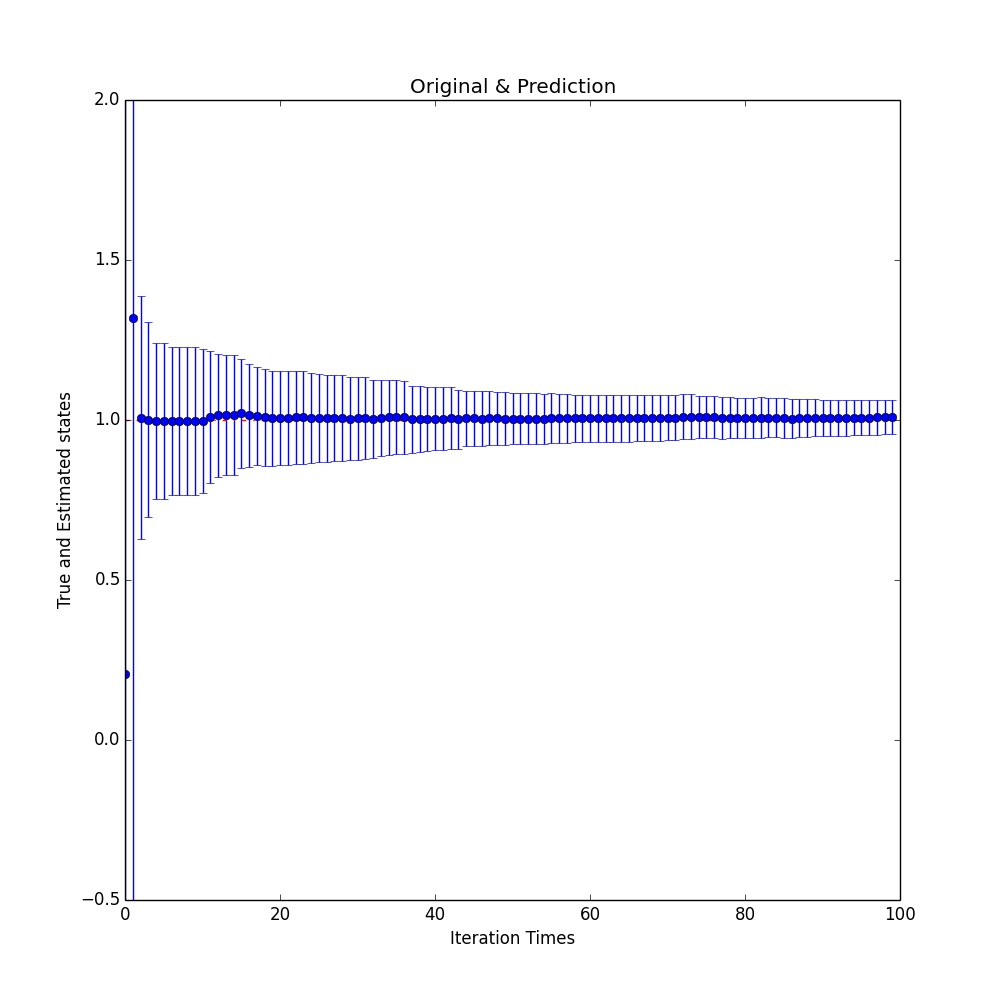
\includegraphics[width=0.9\columnwidth]{kalman}
   \caption{状态 $a$ 的估计。}
  \label{fig:state_a}  
\end{figure}

\section{附录代码}
\label{sec-4}
注意第33行只是简单地将协方差矩阵进行传播,并没有使用时间更新方程。
\begin{verbatim}
 1  # coding=utf-8
 2  import matplotlib.pyplot as plt
 3  import numpy as np
 4  def kalman(A, y):
 5      """
 6      Formulars from the book《Optimal State Estimation》
 7      Page88 & P128
 8      :param A: array in the sklearn form. each "row"
 9       represents an input (the measurement coeffcient).
10      :param y:vector of the response variable (measuremen)
11      :return: x:the estimates. p: covariance of x
12      """
13      dim = A.shape[1]
14      n = A.shape[0]
15      # initialize the estimate of the state(s)
16      # and its(their) covirance
17      x0 = np.zeros((dim, 1))
18      P0 = 1e5 * np.identity(dim)
19      R = 1  # the measurement variance
20      # convert numpy arrays to matrix(suitable for matrix manupulation)
21      x0 = np.mat(x0)
22      P0 = np.mat(P0)
23      # start iteration
24      x, p = [], []
25      for i in range(n):
26          Hk = np.mat(A[i, :][:, np.newaxis]).T
27          Kk = P0 * Hk.T * (Hk * P0 * Hk.T + R).I
28          x_new = x0 + Kk * (y[i] - Hk * x0)
29          Pk = (np.mat(np.identity(dim)) - Kk * Hk) * P0 * \
30               (np.mat(np.identity(dim)) - Kk * Hk).T + Kk * R * Kk.T
31          #Note! this is not universal! We assume that the "time update"
32          #step is trival, i.e., the states are constants
33          #Modify the following line as you need.
34          P0 = Pk                                
35          x0 = x_new
36          # for return
37          x.append(x0)
38          p.append(P0)
39      #convert x back to array
40      x=[np.array(xi).squeeze() for xi in x]
41      return x,p
42  def testKalman():
43      #prepare training data (3-dimension)
44      dataLen = 100
45      A = np.random.random_sample((dataLen, 1)) * 5
46      A = np.c_[A ** 2, A, np.ones((dataLen, 1))]
47      x = np.array([1, 2, 3])
48      y = np.dot(A, x) + np.random.randn(dataLen) * 0.1
49      x_,p= kalman(A, y)
50      print "final estimate:",x_[-1]
51      #extract the confidence interval of the 0th state
52      y_err=[np.sqrt(pi[0,0]) for pi in p]
53      #now plot!
54      fig, ax = plt.subplots(1,1,figsize=(10,10))
55      ax.plot(range(dataLen),np.ones(dataLen)*x[0], 'r-.')
56      # ax.plot(range(dataLen),[xi[0] for xi in x_], 'b-x', alpha=0.5)
57      ax.errorbar(range(dataLen),[xi[0] for xi in x_], yerr=y_err, fmt='o')
58      ax.set_ylim([-0.5,2])
59      ax.set_title('Original & Prediction')
60      ax.set_xlabel(u'Iteration Times')
61      ax.set_ylabel(u'True and Estimated states')
62      plt.show()
63      pass
64  if __name__ == '__main__':
65      testKalman()
\end{verbatim}
% Emacs 24.5.1 (Org mode 8.2.10)
\end{document}

%%% Local Variables:
%%% mode: latex
%%% TeX-master: t
%%% TeX-engine: xetex
%%% End:
